\chapter{提案手法}
\label{chapter:proposal}
低レイテンシなデータセンターの研究動向と, 並列分散処理アプリケーションが生成する特有のトラフィックパターンが引き起こす機能障害をふまえて,
改善手法を提案する.
本提案手法では, 
汎用的なネットワーク機器で構成されたマルチパスなデータセンターネットワークにおいて, エンドノードのみの改良によって, 
長時間継続的にデータを転送し続けるトラフィックが通信している中でのサイズ小さいフロー通信に対する低遅延通信を達成することを目指す.
この目的を達成するために, 提案手法では指向が異なるフローを区別する制御を行うことで, レイテンシ指向なフローについてキューイング遅延を小さくする通信を行う.

\section{Motivation}
提案手法の動機となったのは, MPTCPを用いたデータセンターネットワークモデルである\cite{improving}.
今日のデータセンターネットワークは, FatTreeトポロジーやClosトポロジーに基づいた構成になっており\cite{dctcp, vl2},
等コストな経路が複数存在している. 
提案されたネットワークモデルでは, エンドノードが複数のNICを持ち,
MPTCPによって一つのフローの通信で複数の経路を同時に利用することでスループットを向上させる.
このような複数経路の効率的利用には, IPベースのルーティングで実現しており, それぞれのエンドノードが持つIPアドレスのペアにより, 通信経路が決定する.
現在のMPTCPの実装では, TCPコネクション確立後に互いのIPアドレスを交換し,
新しいサブフローを形成する仕組みになっており, サイズの小さいフローの通信では, サブフローが形成されないまま通信が完結する問題がある. 
その結果, 一つの経路に通信が集中することとなり, で中継スイッチのキューが圧迫され, フローの遅延が大きくなる可能性がある. 
実際, $\S$\ref{reproduction_simulation}での解析でも,
このコネクション確立の際に遅延が生じることが分かっており\cite{mptcp_ana}, どの経路を利用するかによって, 通信性能が大きく変わる.

複数経路の有効活用の手法として, ECMPによるフロー単位でのルーティングがある. 
ECMPではパケットヘッダーの5タプルを用いたハッシュベースのルーティングやラウンドロビンによって, ランダムに経路を選択し, 負荷分散していく. 
この不完全なランダム性のために, ショートフローとロングフローが同一の経路に振り分けられることが起こり,
ショートフローはFCFS(First-Come-First-Serve)方式のキューシステムによって, キューイング遅延が発生する. 
今, Fig.\ref{fig:repflow_scenario}のようなネットワークシナリオを考える. 
このトポロジーは$k=4$ FatTreeトポロジーでのある1ポッド内での通信を示している. 
スイッチS1(S2)と接続されている二つのノードともう一方のノード間にはと二つの等しいコストの経路があり, H2からH4に対してS1-S3-S2の経路を通り,
ロングフローが通信している状況を考える. 
今, H1はH3に対してショートフロー通信を行おうとしたとき, ECMPによるランダムルーティングにより,
$0.5$の確率で同じ経路S1-S3-S2を選択してしまう. 
その結果, ロングフローによるキューイング遅延の影響を受ける. 
実際, $\S$\ref{sec:verification}に示すように実機を用いてこの同一経路を通る問題を検証したところ,
ロングフローをうまく負荷分散した時と同一の経路で通信した時の95パーセンタイル値FCTにおいて,
約10倍程度性能が劣化することが分かった\cite{mptcp_ana2}.

従って, {\bf ロングフローはS1-S3-S2の経路を通り, ショートフローはS1-S4-S2の経路を通るように分散させて通信すること}が,
マルチパス環境における複数経路の効率的な利用の理想的な状況である. 

\begin{figure}[t]
    \begin{center}
    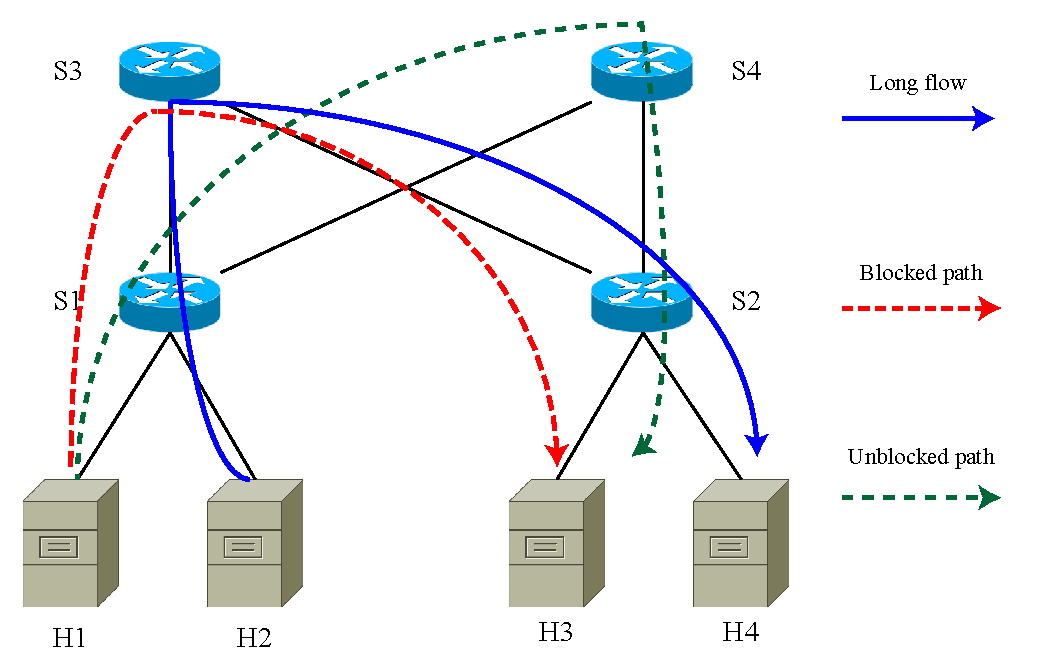
\includegraphics[autoebb, width=250pt]{./img/schenario.pdf}
    \caption{Scenario of queue buildup problem with multi-cost paths)}
    %\ecaption{The control loop in DCTCP}
    \label{fig:repflow_scenario}
    \end{center}
\end{figure}

$\S$\ref{chapter:related_work}に示した既存研究のように, 
データセンターネットワークでのショートフロー問題を解決するために多くの取り組みがされているが, 以下のような要求が考えられる. 
\begin{enumerate}
\item スイッチに対して特殊な実装を施さないこと. 
\item 既存のアプリケーションにも変更なく使えるようにすること. 
\item ショートフローのFCTだけでなく, ロングフローのスループットについても改善すること. 
\end{enumerate} 

1. については, $\S$\ref{chapter:related_work}に示した多くの手法がスイッチに対して変更を加え,
キューイング遅延が起こっている箇所から直接情報を得ることで, 改善を実現している. 
しかし, スイッチに対して変更を加えることで, 全てのスイッチに対してそれらを行う必要性があるため, 実環境への適用に問題があると言える. 
実際, 様々な種類のネットワーク機器が混在している中ではなおさら実現困難である\cite{d3}.

2. については, 既存研究の中でRepFlowは中継スイッチに変更を必要とせず, エンドノード間の変更のみで改善可能な手法であるが,
現状の実装だと, アプリケーションに対する変更が必要であるため, 既存のアプリケーションの変更が必要である\cite{repflow}.
そのため, 実現可能性の観点では有効であるとは言えない. 

3. については, $\S$\ref{sec:verification}に示すように, ロングフローとショートフローが同一の経路で通信を行った場合, 
ECMPによる負荷分散手法では深刻な遅延の問題を引き起こすこととなる. 
$\S$\ref{sec:verification}に示す検証実験では, ショートフローの性能劣化だけでなく,
ロングフローのスループットについても約30\%程度利用率が劣化する結果が得られた. 
RepFlowでは, ショートフローに対して同一の通信を複製することによって, キューイング遅延のない経路を通る,
ショートフローに対して最小のFCTを達成できるという手法であるが, 複製の結果, ロングフローのスループット性能も劣化することが考えられる. 

以上を踏まえて本研究における位置付けを以下のように設定する. 
\begin{enumerate}
\item エンドノード間のみのアプローチで改善を行う.  
\item OSのみに変更を加え, 既存のアプリケーションに変更を加えず適用できる. 
\item フローを指向ごとに区別し, それぞれに応じた改善を行うこと. 
\end{enumerate} 

今, Fig.\ref{fig:repflow_scenario}の環境において上記の前提の下, ロングフローとショートフローを区別し, 別々の経路を通るように分散させて通信することの実現を考える. 
しかし, 既存の技術では{\bf フローの区別}と{\bf それぞれの経路での通信}を達成することができない. 
フローの区別については, 基本的にはフローサイズの大きさで分類することができるが, OSから一つのフローを見た時に,
事前にどのくらいのデータが転送されるかを知る手段はない. 
たとえフローを区別できたとしても, それぞれのフローをどの経路に流すべきか判断するためのメトリックも既存のエンドノードでの技術にはない. 

そこで本研究では, あらかじめ通信経路を決定するために, データセンターネットワーク内に指向毎にレーンを設けるデータセンターレーンモデルと,
フローの指向を区別し, それぞれの経路を切り替えるためのアルゴリズムを提案する. 

\section{Design}
本節では, 本研究における位置付けの下で, 指向毎にフローを区別し, それぞれの経路に切り替えて通信を行うことを実現するため,
データセンターレーンモデルと経路状況を考慮した経路切替アルゴリズムを提案する. 

\subsection{データセンターレーンモデル}
\label{subsec:lane_model}
本小節では, 指向毎にフローを切り替えて制御するためのネットワークモデルとして, データセンターレーンモデルを示し,
そのトポロジーと動作するアーキテクチャについて示す. 

\subsubsection{背景}

今日のネットワーク機器はコモディティ化し, 安価な機器とある用途に特化した高価な機器のコストの差は明確となっており,
データセンター事業者はその性能とコストのトレードオフについて考慮しなければならず,
なるべくコストを抑えたい要求に対して頭を悩ませている\cite{fattree}.
50年以上前の電話網の形成の際にも, 多くの汎用的なスイッチを用いてより多くの端末に接続できるような設計が行われた\cite{clos}. 
そうしたClosトポロジーに基づき,
Ethernetスイッチによって構成されるネットワークトポロジーの一つにFatTreeトポロジーがある\cite{fattree}. 

Full-bisectionalなネットワークトポロジーに対する, 満たすべき要件として以下のようなものが考えられる\cite{improving}.
\begin{itemize}
\item 局所性のないトラフィック
\item すべてのホストが最大帯域活用できる
\item どのアクセスリンクに対してもトラフィックの集中がない
\end{itemize} 
%実際にはこれらの案件が同時に必要となる場合は起こり得ないと考えられ,
%Full-bisectionalな帯域を提供することはコストの面から最適であるとは言いにくい.

今FatTreeトポロジーに対して, 並列分散処理システムを適用させることを考え, Hadoop Distributed File
System(HDFS)によって同じラックの異なるホストにデータを複製し, MapReduceによるmapタスクがそれらに対して割り当てられるとする.
つまり, 同一ポッド内でのトラフィックが発生する.
MPTCPは基本的に複数の経路を持つ コア部分を経由するトラフィックに対して有効に働くが, このように経路選択肢が少ないローカルなトラフィックに対して,
十分に機能しない.

もしすべてのノードに対してMPTCPが実装されたとき, よりMPTCPの特性を引き出すようなトポロジーを検討する必要がある. 
具体的には, エンドノードとToR(Top-of-Rack)スイッチ間のアクセスリンクでボトルネックが発生した時, 効率的な帯域の利用を考える. 
手法として例えば, 1GEthernetリンクから10Gリンクへと変更することでより広帯域なネットワークを実現できるが, コスト面の問題がある. 
また, 従来のSigle-path TCPでは, 1本のリンク容量以上の帯域を得ることはできないという制限がある. 
しかしMPTCPでは, そのような制限はない. 
実際, 近年のサーバ機器には基本的に複数のギガビットイーサネットインタフェースが搭載されており,
エンドノードが二つのNICを持つ際のトポロジーのプロトタイプとして,
Fig.\ref{fig:dual-homing}のようなDHFT(Dual-Homing
FatTree)トポロジーが提案されている\cite{improving}.

\begin{figure}[t]
    \begin{center}
    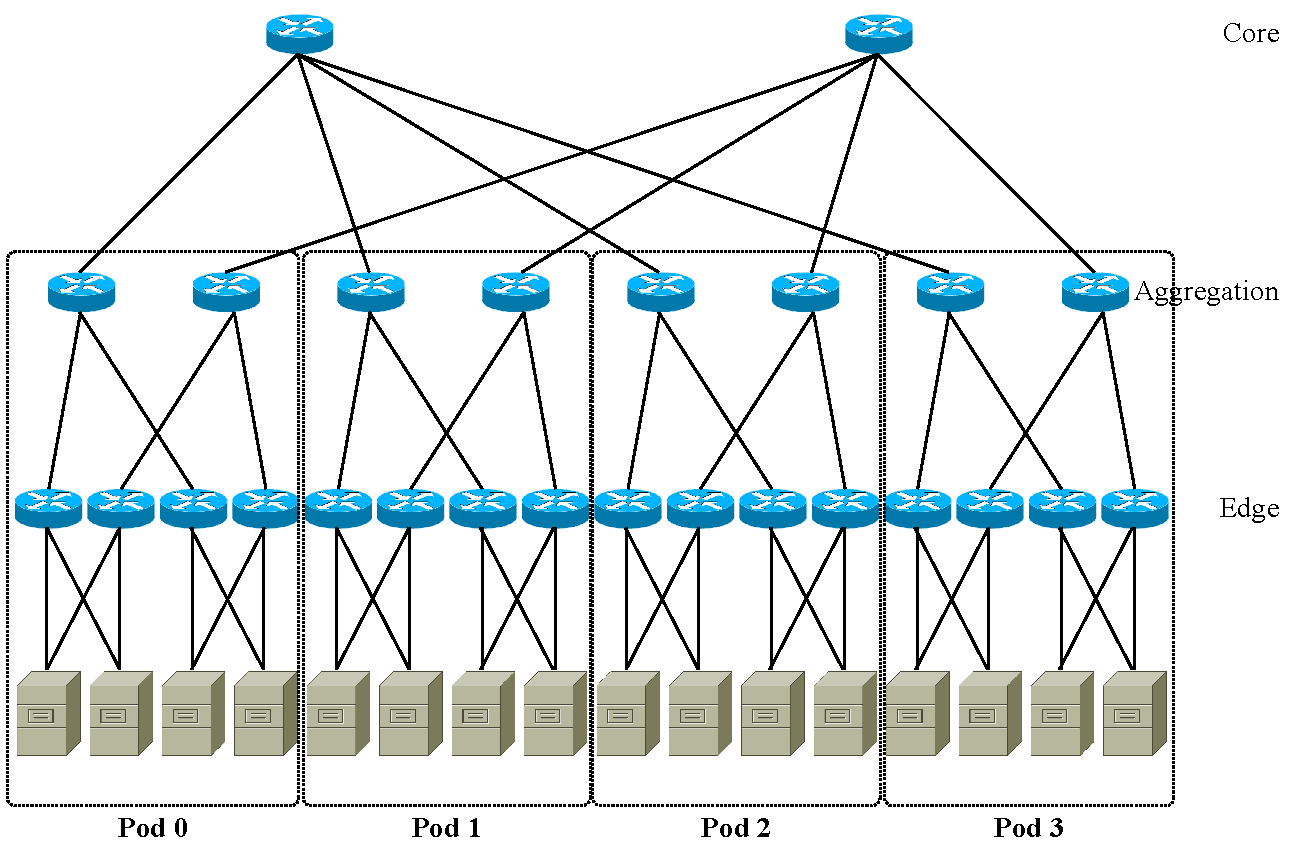
\includegraphics[autoebb, width=250pt]{./img/mhft.pdf}
    \caption{k=4 Dual-homing in the FatTree Topology}
    %\ecaption{The control loop in DCTCP}
    \label{fig:dual-homing}
    \end{center}
\end{figure}

\subsubsection{Motivation}

$\S$\ref{chapter:datacenter_network}にて示したように, 現在のMPTCPの実装では,
まず3ウェイ・ハンドシェイクによってTCPコネクションを確立し, その際にそれぞれの端末がMPTCPを利用可能かどうかのネゴシエーションを行う.
MPTCPが利用可能な場合, 互いの持っているIPアドレスを交換し(add\_address), その後サブフローを形成し, 複数の経路利用しながら通信を行う. 
その時MPTCPの輻輳制御によって, それぞれの通信状況に合わせてウィンドウサイズが調整され, 通信される\cite{balia}. 
しかし, 今のMPTCPではサイズの小さいフローについては, サブフローを形成する前に通信が完了する. 
そのため, たとえTCPコネクションを形成するための経路が混雑した状況であっても, MPTCPによってその経路を回避する手段はなく,
Fig.\ref{fig:repflow_scenario}で示したような性能劣化を導いてしまい,
マルチパス環境における複数経路の効率的な利用を実現できなくなる. 
ここで, 現状MPTCPを用いて経路選択をする上での課題を以下に示す. 
\begin{enumerate}
\item 基本的なIPベースのルーティングでは, コネクションを確立する経路は毎回同じである. 
\item あらかじめ経路を決定するには, 通信経路の輻輳状況を事前に把握しておく必要がある. 
\end{enumerate} 
1. についてはIPベースのルーティングでは基本的に宛先アドレスと送信元アドレスから決定されるので、コネクションを確立するアドレスペアが同じだと,
それに従い通信経路も同じものが選択される. 
異なる経路を選択するためには, 宛先アドレスとしてサーバ側の持つアドレスを事前に把握しておく必要があり,
その上でECMPやラウンドロビンのような分散手法の適用が考えられる.
しかし先に示したように, これらの分散手法では完全な負荷分散は実現できず, あらかじめ通信状況を取得するなどのアプローチが必要である. 

2. については, 本研究ではエンドノードに対する変更のみで改善を目指しているため, 遅延している中継スイッチから, 直接情報を得ることはできない. 
これまでの通信状況を把握しておくための取り組みとして, OpenFlowを用いた手法が提案されているが,
経路の統計情報を得るためのオーバーヘッドが発生するため, 現実的な解決策とは言えない\cite{devoflow}.

これらを踏まえて, 用途の異なるフローに対して通信経路を切り替えるため, データセンターレーンモデルを提案する.

\subsubsection{アーキテクチャ}
複数のインタフェースを持つエンドノードに対してFatTreeトポロジーを用いて, 指向毎のフローを切り替え制御の実現を目指す.  
具体的には複数の等価コストな経路に対してレーンを定義し, 区別したフローに対して通信を行う経路を設置する. 

このモデルの狙いは, スイッチから直接情報を得るような粒度の細かい制御を用いて遅延を回避するのではなく,
あらかじめ通信すべき経路を区別しておくことで, それぞれの目的にあった通信を実現することにある. 
データセンターレーンモデルでは, 以下のような用途のレーンが設置される. 
\begin{itemize}
\item {\it Query traffic}や{\it Short message
traffic}のようになるべく短いFCTで通信したいショートフロートラフィックに対しては, レイテンシ指向なフローとみなし,
常に空いている状態に保たれたショートフローレーンSL(Short-flow Lane)を用いる.
\item {\it Backgroung traffic}のようにより大きなスループットで通信したいロングフロートラフィックに対しては,
スループット指向なトラフィックとみなし, 一般に複数の経路が設置してあるロングフローレーンLF(Long-flow lane)を用いる. 
\end{itemize}

Fig.\ref{fig:lane_model}にネットワークレーンモデルを示す. 
今, 互いのエンドノードはそれぞれのインタフェースごとにIPアドレスを持っているとし, それぞれ$Lane Info$が与えられているとする. 
この$Lane Info$の値は, 各ノードのOSに対して設定するパラメータであり, 各ノードが保有している送信元アドレスと1対1に紐付いている. 
% このとき, 中継するスイッチでは各インターフェース毎に経路を分散されることが望ましい.  
これにより, 初めのTCPコネクションを形成する$src:10.1.0.1, dst:10.2.0.1$の通信に対しては, Path1でコネクションを形成し, 
次に, 互いのアドレス$(10.1.1.1, 10.2.1.1.)$を交換し, サブフローを形成できる状態にする. 
サブフロー$src:10.1.1.1, dst:10.2.1.1$の通信に対しては, Path2を利用される. 
このように, それぞれのサブフローの通信においては, 異なる経路を形成し, 通信が行われる. 
従って, 送信元アドレスが決定した時点で, 通信経路が決定するため, 送信元アドレスと紐付いている$Lane
Info$が通信経路のレーンを示していることになる.

\begin{figure}[t]
    \begin{center}
    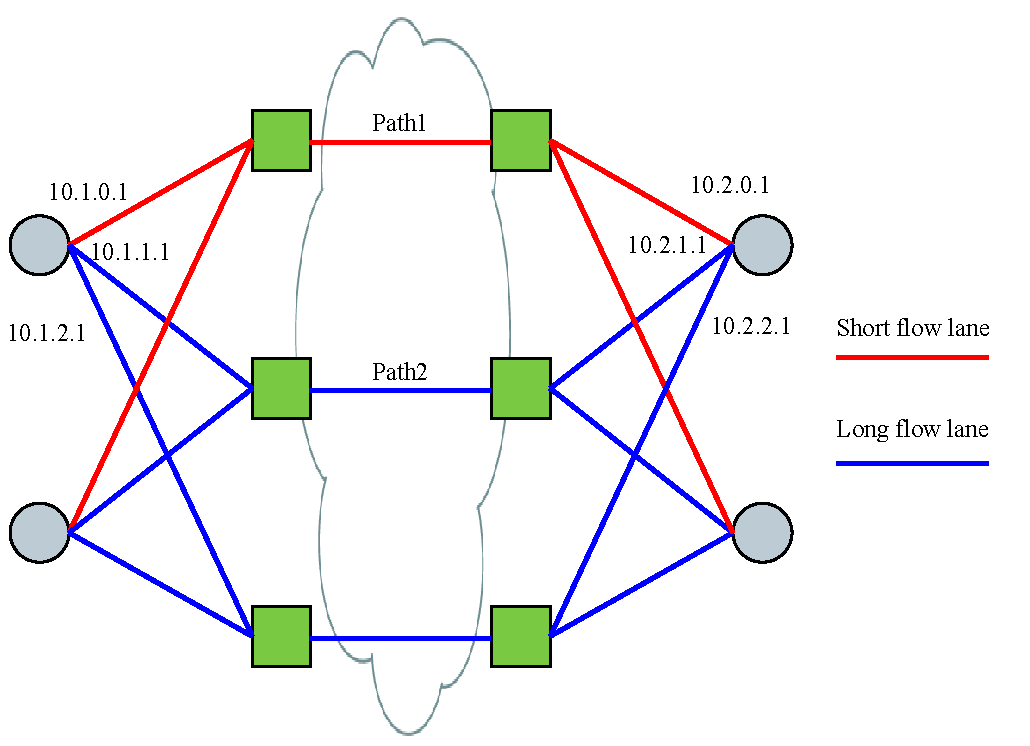
\includegraphics[autoebb, width=250pt]{./img/lane_model.pdf}
    \caption{Datacenter Lane Network Model}
    %\ecaption{The control loop in DCTCP}
    \label{fig:lane_model}
    \end{center}
\end{figure}

\subsection{経路切り替えアルゴリズム}
次に, $\S$\ref{subsec:lane_model}にて示した, データセンターレーンモデルに対して, フローを指向毎に区別し, 
経路切り替えるアルゴリズムを示す.
\subsubsection{モチベーション}
今回のエンドノードOSのみのアプローチでは, フローサイズを用いた区別はアプリケーションに対する変更が必要となり, 現実的な解決方法ではない. 
そこで提案するアルゴリズムでは, 区別ためのメトリックとしてフロー持続時間を用いることで, SLを輻輳のない状態に保ち, フロー持続時間の長いものについては,
LLに切り替えることで, それぞれの指向を最大限達成することを実現する. 
特にSLについては, ロングフローによるキューイング遅延が抑えられるため, FCTを短縮することができるように設計している. 

先にも述べた通り, 通信経路は送信元アドレスと, 宛先アドレスによって決定され, 基本的にはTCPコネクションを形成する通信経路は毎回同じものになり,
また, フロー持続時間を用いて区別を行う手法であるために, 通信開始当初はフローの区別をすることができない. 
そのため, 提案するアルゴリズムでは, 以下のような動作により,
通信開始時にはすべてのフローがレイテンシ指向なフローと判断され, その後ロングフローの場合区別が行われる. 
以下に通信経路の切り替えの流れを示す
\begin{enumerate}
\item SLに対してTCPコネクションを形成する
\item 互いの持つアドレスを交換し合い, サブフローを形成する
\item サブフローを形成した際, 送信元アドレスの$Lane Info$がLLであれば, cwnd=1を代入する. 
\item アルゴリズムがフローをロングフローであると判断すれば,  SLのサブフローに対してcwnd=0を代入し,
LLのサブフローに対して設定されている輻輳制御のアルゴリズムを適用する
\end{enumerate} 
サブフローを形成した際に, cwnd=1の小さい通信を行うことで経路の状況を取得する. 

\subsubsection{実装上の課題}
上記のような経路切替アルゴリズムを実現するための実装上の課題がある. 

\underline{$\cdot$ どのようにフローを区別するのか} \\
先に示した通り, データセンターのアプリケーショントラフィックを考えたときに, それぞれの用途によって指向が異なる. 
既存研究ではフローサイズ($\geq 100KB$)をメトリックとして区別\cite{repflow}を行っていたが,
現状の実装だとカーネルにおいては通信開始時点でフローサイズを把握することはできない. 
そのため本提案手法では, 指向区別のための主なメトリックとして`` フロー持続時間''を用いる.
% これにより, 例えば最も単純な手法においては, フロー持続時間を直接用いて, それを越えた時間通信するフローをレイテンシ指向なロングフロー,
% それ以内に完結するフローをショートフローと仮定して制御を行う. 

\underline{$\cdot$ いつ経路を切り替えるのか} \\
フロー持続時間のデッドライン時間を用いた最も単純な手法として, 例えば300[ms]と設定することで,
300[ms]を越えた時点でフローの切り替えが行われるような制御が考えられる. 
しかし, SLが混雑しているにもかかわらず, SLで持続して通信を行うことや, LLが混雑しているにもかかわらず,
デッドライン時間を超えると経路が切り替わる状況も想定されるため, このような単純な手法だと経路の状況によっては改善が見込めない. 
そのため, 経路状況に対応し経路を切り替えるためのメトリックとして`` リンクコスト''を定義し, リンクコストベースの経路切り替え手法を提案する. 

\subsubsection{リンクコストベースの経路切り替え手法}

提案するリンクコストベースの経路切り替え手法によるトラフィック制御では, スイッチ, エンドノードに対してそれぞれのキューの混雑具合を考慮し,
経路を制御する.
本質的な狙いは, フローサイズに従って通信が終えるということであり, 具体的には,
フローサイズの大きいロングフローが通信している中でショートフローが発生した場合,
ロングフローが占有しているキューを避けた経路をショートフローが利用することでフロー完結時間の短縮化を実現するものである.

\underline{$\cdot$ RTT(Round-Trip Time)$\tau(t)$モデル化} \\
通信における遅延において, 様々な要因が考えられるが, 経路状況によって変動し. 最も遅延の影響が大きい要素として,
キューイング遅延がある\cite{RTT_est, queue_delay}.
今クライアントノードでのACKパケットを受けた時のRTTを$\tau(t)$とする. 
この時, $d_{l, i}(t)$はリンク$i$におけるリンク伝送遅延, $d_{p, i}(t)$は伝搬遅延, $d_{q,
i}(t)$はキュー遅延を表している. 
この時, エンドノード間の経路として$m$個のネットワーク機器を介する時, 以下のような式でRTTを表現できる. 
\begin{eqnarray}
\tau(t) = \sum ^m _{i=1} \Bigl(d_{l, i}(t) + d_{p, i}(t) + d_{q, i}(t)  \Bigr)
\end{eqnarray}
一般にセッションの間, ネットワーク内の経路は安定して通信を行うと想定することができ, 伝送遅延$d_{l, i}(t)$と伝搬遅延$d_{p,
i}(t)$は定数としてみることができ, それらを併せてRTTに対するバイアスとしてみることができる\cite{RTT_est}. 
そのため, RTTが変化する最も大きな要因の一つは, 経路ごとのキューイング時間の変化であると考えられる. 

キューイング時間の変化を最も単純なモデル式で表すと, ノード$i$におけるキュー長$q_i(t)$とリンク容量$c_i$を用いて,
ノード$i$での時間$t_i$での$d_{q,i}(t)$はキュー遅延を以下のように表現することができる. 
\begin{eqnarray}
d_{q,i}(t) = \frac{q_i(t_i)}{c_i}
\end{eqnarray}
これによりACKパケットを受け取った時の時刻$t$におけるRTTは以下のように簡単化される. 
\begin{eqnarray}
\tau(t) = \sum ^m _{i=1} \frac{q_i(t_i)}{c_i} + bias
\end{eqnarray}

\underline{$\cdot$ SL, LLに対するリンクコスト} \\
ここで$\tau_0$は最小RTT, $d_0$は最小キュー遅延を用いて, キューイング遅延の変化量である相対キュー遅延$\nu(t)$を以下のように表す. 
\begin{center}
\begin{eqnarray}
\nu_{i}(t) &=& \tau(t) - \tau_0 \\
&=& \Bigl( \sum ^m _{i=1} \frac{q_i(t_i)}{c_i} + bias \Bigr) - \Bigl( \sum
^n_{i=1} \frac{q'_i(t_i)}{c_i} + bias \Bigr) \\
&=& d_t -d_0
\end{eqnarray}
\end{center}
この$\nu(t)$が通信経路の状況を表すと仮定し,
これをパラメータとしたリンクパフォーマンス関数\cite{bpr}としてリンクコストを以下のように定義する.
リンクコストについては, Davidson関数を参考に導出した\cite{bpr, davidson}.

\begin{eqnarray}
\label{linkcost}
\left\{
\begin{array}{l}
t_{a}^{SL} = t_0 \cdot \bigl\{ 1 + \alpha \cdot \nu(t)^\beta \bigr\} +
{\rm sgn} (t - t_{deadline}) \cdot \gamma (t - t_{deadline})^\delta \\
t_{a}^{LL} = t_0 \cdot \bigl\{ 1 + \alpha \cdot \nu(t)^\beta \bigr\} 
\end{array}
\right.
\end{eqnarray} 
ここで, $t^{SL}_a(t), t^{LL}_a(t)$はそれぞれSL, LLのリンクコスト値であり, $t_0$は最小リンクコスト,
$sgn(t)$は符号関数, $t_{deadline}$はデッドライン時間, $\alpha \sim \delta$はパラメータである.
一般に, このリンクコスト関数の変数, パラメータの性質はTable.\ref{table:link_cost_nature}のように表さる
このリンクパフォーマンス関数を用いた, 通信経路切り替えアルゴリズムをAlgorithm \ref{alg1}に示す. 
このアルゴリズムによって, サブフローが形成された際に, デッドライン時間$t_{deadline}$が設定され(Initialization),
ACKパケットが届き, TCPスタックによるRTTの推定がされた時にコスト計算され(Calculating link-cost),
それぞれのサブフローのリンクコストとの比較を行い(Judging Phase), SLのコストがLLよりも大きくなった場合,
LLの方が有利に通信ができると判断され($judge_flag \Leftarrow 1$), SLのウィンドウサイズを0に,
LLのウィンドウサイズを設定している輻輳制御アルゴリズムに従って算出された値を適用する. 
SLのコストがLLよりも小さいままの場合, SLのウィンドウサイズは輻輳制御に従い, LLのウィンドウサイズは1に設定される. 
これは, LLの用いる通信経路の状況を把握するため, 非常に小さなパケットを流しRTTを推定するためである. 


\begin{table}[t]
    \begin{center}
    \caption{The Natures of the parameter and variables in Link Cost Function}
    \begin{tabular}{|c|c|}
    \hline
    Variables, Parameter & Nature \\ \hline \hline
    $\alpha$ & \parbox{25zw}{リンクコスト関数の立ち上がりの速さを示す. $\alpha$が小さい場合,
    キューイング遅延の影響が大きくなってもあまりRTTが増加しない }\\ \hline
    $\beta$ & \parbox{25zw}{リンクコスト関数の傾きの度合いを示す.
    経路の通信環境が悪化し$\nu$が大きくなる領域は$\beta$の影響が支配的になる領域である.
    $\beta$が大きいと混雑に対する感度がよりアグレッシブな挙動を示す. } \\ \hline
    $\gamma$ & \parbox{25zw}{デッドライン時間$t_{deadline}$へ近づく速さを示す. $\gamma$が小さい場合,
    デッドライン時間を設定することによるSLの優位性が小さくなる. }\\ \hline
    $\delta$ &
    \parbox{25zw}{リンクコスト関数のデッドライン時間$t_{deadline}$に近づく傾きの度合いを示す.
    $\delta$が大きいとよりデッドライン時間に対する影響が強くなり, 通信状況よりもデッドライン時間に対する挙動の影響が大きくなる. } \\ \hline
    $sgn(t-t_{deadline})$ &
    \parbox{25zw}{リンクコスト関数のデッドライン時間$t_{deadline}$を超えるまでの挙動の違いを示す. デッドライン時間を超えない時間では,
    上に凸の関数をとなり, デッドライン時間を超えると下に凸の挙動を示し, デッドライン時間を超えた時の増加の速さが大きくなり,
    デッドライン時間に対する影響が大きくなる. }
    \\
    \hline
    \end{tabular}
    \label{table:link_cost_nature}
    \end{center}
\end{table}


\begin{algorithm}
\caption{Caluculating link-cost}
\label{alg1}
\begin{algorithmic}[1]
\STATE $\triangleright $ \underline{Initialzation}
\STATE $t_{deadline} \Leftarrow now + THRESHOLD$
\STATE $\tau_0 \Leftarrow 0$
\STATE $t_{0} \Leftarrow 1$
\STATE $\triangleright $ \underline{Receiving ACK packet:Calculating link-cost}
\STATE $j = $ which subflow the ACK is
\STATE $RTT_j = $ RTT estimation by TCP stack with smoothing
\STATE $measurement\_cost = $ Calculating link-cost
\STATE $cost_j \Leftarrow 3/4  \ast cost_j + 1/4 \ast measurement\_cost$
\COMMENT {Updating cost value with smoothing}
\STATE $base\_RTT = $ Updating if the RTT is the smallest one
\STATE $base\_cost = $ Updating if the cost is the smallest one
\FOR{$i=0$ to $SUBFLOW\_NUMBER$}
\STATE $Min\_Cost's Lane \Leftarrow$ Detecting lane\_info of minimum cost(LL
or SL)
\ENDFOR
\STATE $\triangleright $ \underline{Judging phase}
\IF {$Min\_Cost's Lane$ is LL(Long-flow Lane)}
\STATE $judge\_flag \Leftarrow $ 1
\COMMENT {Change subflow's state}
\ENDIF
\IF {$judge\_flag = 1$}
\STATE {$\triangleright$} \underline{Switching phase}
    \IF {$lane\_info = 1$}
    \STATE $cwnd \Leftarrow 0$
    \COMMENT {This subflow in SL}
    \ELSE
    \STATE $cwnd \Leftarrow $ tcp\_congestion\_control
    \COMMENT {This subflow in LL}
    \ENDIF
\ELSE
\STATE {$\triangleright$} \underline{Keeping state phase}
    \IF {lane\_info = 1}
    \STATE $cwnd \Leftarrow $ tcp\_congestion\_control
    \COMMENT {This subflow in SL}
    \ELSE
    \STATE $cwnd \Leftarrow 1$
    \COMMENT {This very small traffic in LL for probe }
    \ENDIF
\ENDIF
\end{algorithmic}
\end{algorithm}

\section{Discussion}

\subsection{利点}
提案手法は, $\S$\ref{sec:expected_effect}に示す性能障害を次のように解決する. \\
{\bf Queue buildup}\\
提案手法では, デッドライン時間, リンクコスト値を用いてロングフローであると判定された場合, 速やかにSLへとトラフィックが移行する. 
これにより, SLはレイテンシ指向なショートフローに対して, 通信経路を良好な状態に保つことができ, FCTを短縮化される. 
また, ロングフローに対しても, ショートフローによって輻輳状態となったLLを避けて通信することができるため, スループットの改善が期待できる. 

しかし実質的には, フローの種類が未知である通信発生時については, すべてのフローがSLで通信される. 
このため, ショートフローが短時間に大量に発生した場合や, ロングフローとショートフローが同時に通信を開始した場合には, 通信性能が劣化することが考えられる. 


\subsection{アルゴリズム実装の検討}
提案手法では, 通信可能なすべてのサブフローに対して通信状況を表すリンクコストを計算し, 通信経路を切り替える際のメトリックとして用いる. 
その際, 最も重要な変数の一つはRTTである. 
今回の提案手法では, RTTの推定にはTCPスタックのtcp\_rtt\_estimator用いる.
この推定結果を用いてリンクコストの計算を行うが, RTTや前のパケットの到着時間の差分の揺らぎによっては, リンクコスト値も大きく変動する. 
そのため, リンクコストの平滑化を行う(Line 9). 

また通信開始時のSLでの通信の際にも, LLのリンクコストを計算する必要があるため, LLでのウィンドウサイズを1に設定し,
小さなトラフィックを流す(Line 31).
これにより, すべての経路について経路状況を見ることができ, 経路状況に合わせた制御をすることができる. 

